\section{GPGPU Computing}

Originariamente le Graphics Processing Units (GPU) sono state concepite
come co-processori il cui scopo
era puramente l'elaborazione grafica, mentre le altre funzionalità
non strettamente legate a questo ambito erano gestite dalla 
Central Processing Unit (CPU).
In seguito si è diffuso l'utilizzo del parallelismo fornito dalle GPU
per accelerare diversi tipi di software non riguardanti
l'area della computer grafica, dando luogo al General-Purpose computing
on Graphics Processing Units, cioè l'utilizzo di questo tipo di hardware
per applicazioni non legate all'elaborazione delle immagini.
Sebbene le GPU operino a frequenze molto inferiori rispetto alle CPU, il loro
punto di forza risiede nella presenza di molte più unità di elaborazione
(denominate core), in grado quindi di eseguire centinaia o migliaia di thread
in parallelo rispetto all'esiguo numero disponibile per la CPU.
La tipologia di thread
istanziabile dalla GPU è ottimizzata per garantire un basso overhead
per quanto riguarda la loro creazione e uno scambio di contesto quasi
istantaneo, evitando così un decadimento delle presentazioni dovuto al cospicuo
numero di thread generalmente sfruttati per risolvere un determinato task
\cite{kirk2007nvidia}.
\\
In generale ad uno stream di dati di input corrisponde la creazione di un
numero finito di thread per elaborare le informazioni ricevute e solitamente
ogni thread esegue le medesime istruzioni applicate ad un sottoinsieme
dei dati. Un'architettura che opera secondo questo concetto è stata
classificata da Michael J. Flynn con il termine di Single Instruction, Multiple 
Data (SIMD)\cite{duncan1990survey} e prevede
la presenza di un'unità centrale di controllo (in questo caso la GPU) che
distribuisce le istruzioni da eseguire alle unità di elaborazione (i thread).
Queste unità possono accedere alle informazioni attraverso una comunicazione
del tipo processo-processo oppure processo-memoria come nel caso delle GPU.
\\
In ambito scientifico l'architettura SIMD è stata utilizzata per la simulazione
di fenomeni fisici, chimici e biologici oltre che all'elaborazione delle
immagini, grazie al fatto che le singole unità di elaborazione svolgono
operazioni anche in virgola mobile con indirizzamento sia a 32 che a 64 bit.
\\
Oltre a SIMD è stata definita anche un'architettura che prevede
l'esecuzione di diverse istruzioni su diversi stream di dati, denominata
Multiple Instructions, Multiple Data (MIMD)\cite{duncan1990survey}.
Questa architettura viene utilizzata solamente quando le unità di elaborazione
devono eseguire istruzioni eterogenee, dunque è necessaria la presenza
di diverse unità di controllo hardware.
Essendo la decentralizzazione un punto cardine
di questo paradigma, è necessario introdurre anche il concetto di
sincronizzazione fra processi, utilizzando lo scambio di messaggi o
la memoria condivisa, dato che le macchine operano in modo asincrono.
\\
Quindi per quanto riguarda l'elaborazione di insiemi di fenomeni del mondo reale
che obbediscono tutti alle medesime leggi,
risulta opportuno utilizzare il paradigma SIMD, dato che è più semplice da
implementare e gestire.

\begin{figure}[H]
    \begin{minipage}[b]{.5\linewidth}
        \centering
        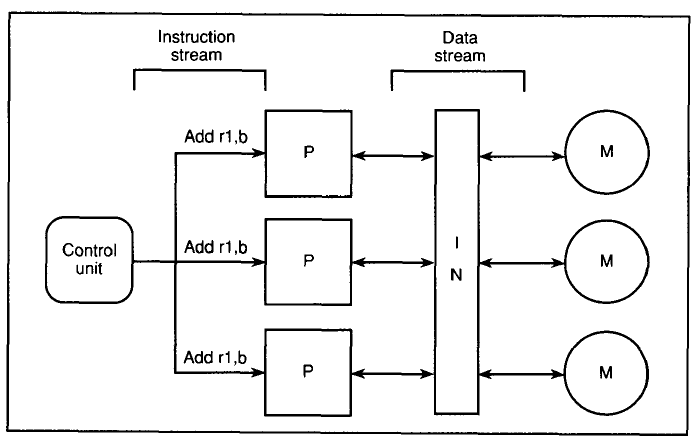
\includegraphics[scale=0.3]{simd}
        \subcaption{Architettura SIMD}
    \end{minipage}
    \begin{minipage}[b]{.5\linewidth}
        \centering
        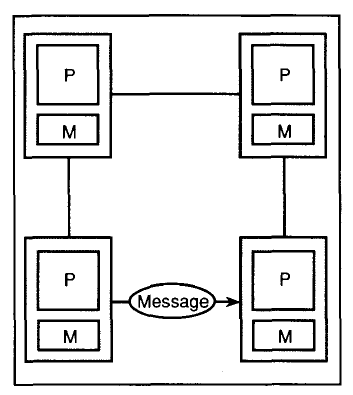
\includegraphics[scale=0.4]{mimd}
        \subcaption{Architettura MIMD}
    \end{minipage}
    \caption{Schemi di esecuzione di architetture SIMD e MIMD}
    \label{fig:simd-mimd}
\end{figure}

La figura \ref{fig:simd-mimd} mostra i due diversi schemi di esecuzione
delle architetture definite in precedenza, dove con $P$ è indicato il processore
e con $M$ la memoria. Da notare il fatto che, come spiegato precedentemente,
lo schema SIMD prevede che l'unità di controllo distribuisca ai processori $P$
lo stream di istruzioni da eseguire elaborando le informazioni
provenienti dallo stream di dati, utilizzando anche la memoria $M$ come supporto
per lettura e scrittura di informazioni. Mentre nello schema MIMD si nota
il diverso approccio adottato rispetto a SIMD, ovvero l'assenza di un'unità
di controllo centrale e ogni processore $P$ che esegue
unp stream di istruzioni differente l'uno dall'altro,
con possibilità di accesso solamente alla
propria memoria $M$ dedicata e con sincronizzazione e scambio di informazioni
tra processori mediante lo scambio di messaggi, sottolineando maggiormente
la natura asincrona di questo modello.

Sebbene le GPU aumentino le performance in maniera considerevole, questi
vantaggi si ottengono nel momento in cui lo stream di dati assume
una dimensione tale per cui l'overhead di creazione dei thread risulti
irrisorio rispetto alla computazione che si deve andare ad effettuare.
Ad esempio nel momento in cui vogliamo effettuare la ricerca di un valore
specifico all'interno di un array, se la dimensione dell'input è di poche
migliaia di elementi l'utilizzo della GPU risulta inutile poichè
le moderne CPU possiedono frequenze elevate che favoriscono l'esecuzione
di istruzioni sequenziali su insiemi di pochi elementi, mentre l'istanziamento
di un basso numero di thread unito ad una frequenza delle unità di elaborazione
della GPU molto inferiore rispetto a quella delle CPU non favorisce un
approccio parallelo alla risoluzione di questo tipo di problemi.
